\problemname{Tycho}

\illustration{.4}{img/MarsPerseveranceRover.jpg}{}

\noindent
The planetary exploration vehicle \emph{Tycho VIII} needs to get back to the home base after collecting mineral samples.
Tycho travels in a straight line from position~$0$ to the home base at position~$b$.
While moving, it advances at a slow but steady pace of $1$~unit per second.
Every second, Tycho takes $1$~unit of environmental damage from the harsh planetary conditions.

The situation is made even worse by radiation from a nearby pulsar, which adds $d$ additional units of damage every $p$ seconds.
However, the radiation damage can be avoided by seeking shelter in one of $n$ different hiding spots---caves, vegetation, large rocks, carcasses of the planet's megafauna---along the way.
Tycho can choose to stand still at any point for any integer number of seconds.

The starting position~$0$ and the home base at~$b$ are both sheltered, so Tycho takes no radiation damage there.

\medskip
What is the minimum damage Tycho will take on its journey back to the home base?

\section*{Example}

Consider the situation where the home base is at position $18$ and there are shelters at positions $8$ and $15$.

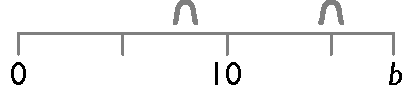
\includegraphics[width=.3\textwidth]{img/samplesetup}

Assume that the pulsar's period is $4$, so unsheltered Tycho would take damage at times $4$, $8$, $12$, etc.
If Tycho leaves from the starting position (where it's sheltered) at time $0$, it can reach the first shelter after $8$ seconds, incurring radiation damage $d$ at time $4$ (but none at time $8$ because it's sheltered then).
Continuing without stopping, it reaches the home base at time $18$, incurring $d+d$ more units of radiation damage (at times $12$ and $16$, respectively).
This way it incurs $d+d+d=3d$ units of radiation damage and $18$ units of environmental damage.
If instead Tycho waits at the $2$nd shelter (at position $15$) for $1$ second, the pulse at time $16$ causes it no damage, and it reaches the home base at time $19$ with a total of $2d + 19$ units of damage.
This is better for most values of $d$.
The two situations are shown here:

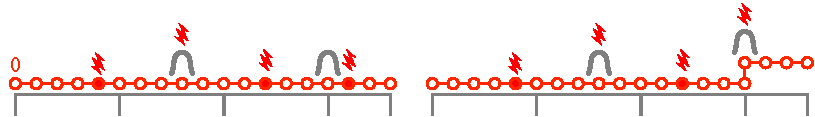
\includegraphics[width=.8\textwidth]{img/sample1_2.pdf}

If the pulsar's period is $10$, Tycho can wait at the starting position for $2$~seconds and then just go home without stopping at any shelter.
Thus it passes the $1$st shelter (at position~$8$) at just the right moment when the pulsar flares and arrives at the home base at time $20$, for a total of $20$ environmental damage and no radiation damage at all.

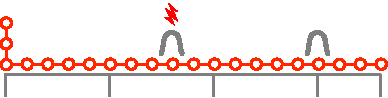
\includegraphics[width=.4\textwidth]{img/sample3.pdf}

\section*{Input}

The first line consists of four integers $b$, $p$, $d$, and $n$, separated by single spaces:
the location $b$ of the home base,
the pulsar's flare period~$p$,
the additional radiation damage~$d$ caused by each flare of the pulsar,
the number~$n$ of the shelters.
The following $n$~lines each contain an integer giving the shelter locations $a_1$, $\ldots$, $a_n$, with 
$0<a_1<\cdots <a_n< b$. % constraint:shelterbounds, constraint:sortedshelters

\section*{Output}

Print a single integer: the minimum amount of damage Tycho must take to reach $b$.

\section*{Constraints and Scoring}

You can assume
$p < b$ % constraint:pulsehappens
and
$n < b$. % constraint:sheltersfit
We always have
$1\leq b\leq 10^{12}$, % constraint:b
$0\leq d \leq 10^6$, %constraint:d
and
$0\leq n \leq 10^5$. % constraint:n

Your solution will be tested on a set of test groups, each worth a number of points.
Each test group contains a set of test cases.
To get the points for a test group you need to solve all test cases in the test group.
Your final score will be the maximum score of a single submission.

\medskip
\begin{tabular}{lll}
Group & Points & Constraints \\\hline
  $1$ & $8$  & $p\leq 10^6$ and Tycho does not need to wait \emph{after} leaving position~$0$.$^*$ \\ % constraint:nowait
  $2$ & $5$  & $b\leq 1000$, $p\leq 100$, $n\leq 10$ \\
  $3$ & $7$  & $b\leq 1000$ \\
  $4$ & $15$ & $p\leq 10^6$, $n\leq 1000$\\
  $5$ & $20$ & $p\leq 100$\\
  $6$ & $35$ & $p\leq 10^6$\\
  $7$ & $10$ & \emph{No additional constraints}
\end{tabular}

\medskip
\noindent $^*$ In test group~$1$, Tycho may still need to wait at position~$0$ \emph{before} it starts moving.
For example, sample inputs $2$, $3$, and $4$ belong to test group~$1$.
